%DO NOT MESS AROUND WITH THE CODE ON THIS PAGE UNLESS YOU %REALLY KNOW WHAT YOU ARE DOING

\chapter*{ Final Product }
\addcontentsline{toc}{chapter}{Final Product }
\noindent Lusso ( Luxury in Italian ) is a great grinder, with a speedy, durable burr set and consistent grinding performance. It looks and feels solid, it has a timer switch that makes it easy to grind the exact same amount of coffee each time you brew. It also has a sturdy base which helps keep burrs from vibrating out of calibration. Lusso will cost 199 Euro only.
\begin{figure}[h]
    \begin{minipage}[c]{.6\textwidth}% or {.6\linewidth}, it's the same here
       \begin{tabular}{|c|c|} 
 \hline
 \multicolumn{2}{|c|}{Specifications} \\
 \hline\hline
 Number of settings & 40 \\ 
 \hline
  Burr Type & Conical burr grinders \\
 \hline
 Compatible with & Both beans and pods \\
 \hline
 Warranty & 1 year \\
 \hline
 Dimensions & 12x35x16 cm \\
 \hline
 Grinding speed & 450 RPM \\
 \hline
 Bean Hopper Capacity & 8 oz (227g) \\
 \hline
 Weight &  7 lbs. (3.1kg) \\
 \hline
 Power &  AC Supply 110 V or 220-240V \\
 \hline
 \end{tabular}

    \end{minipage}
    \hfill
    \begin{minipage}[c]{.5\textwidth}
        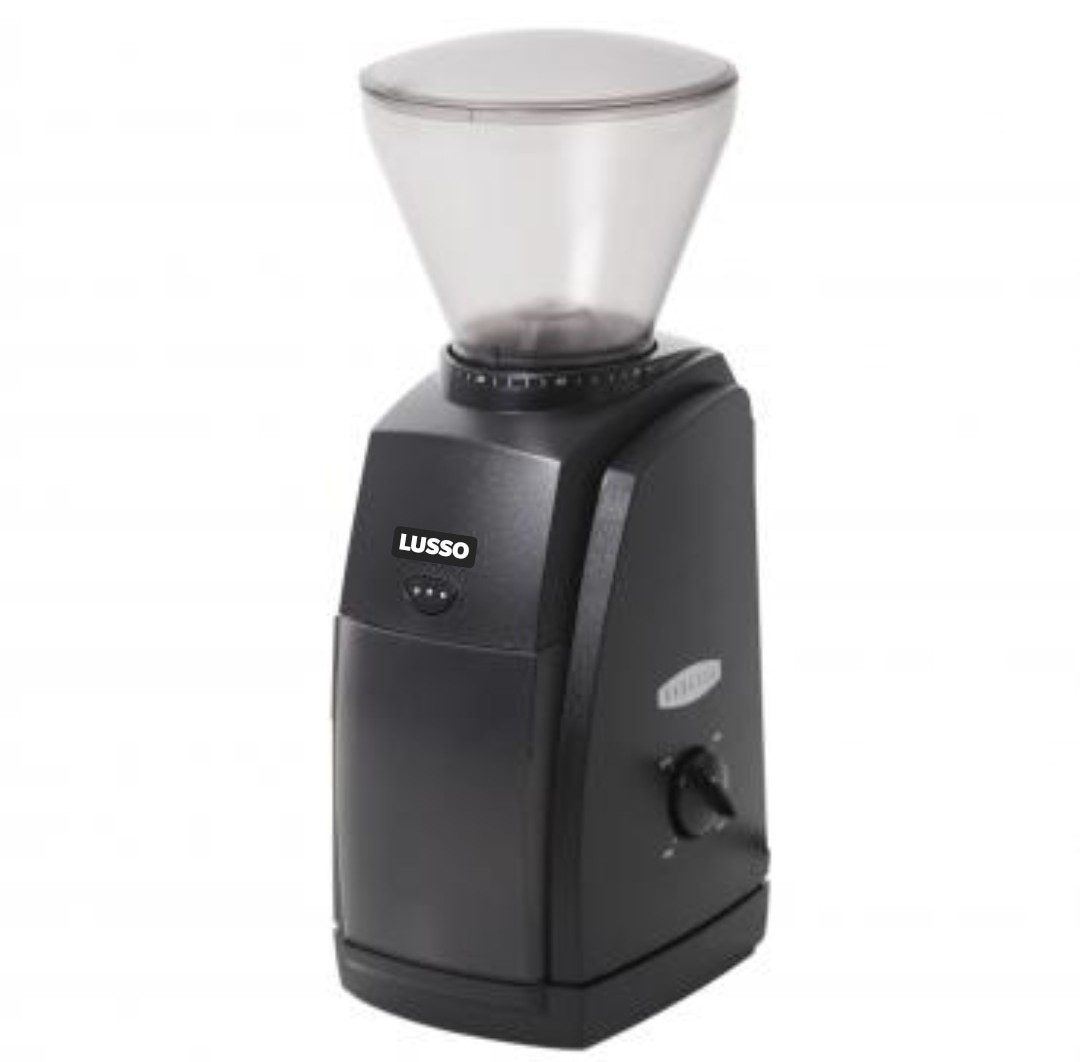
\includegraphics[width=\linewidth]{grinder.jpg}% caution: here you cannot replace \linewidth by \textwidth, since within this minipage, \linewidth=.3\textwidth
    \end{minipage}
\end{figure}      


